% !TeX spellcheck = en_US
\chapter{IceAct Parameterization}

The simulation results discussed in chapter \ref{chap:simresults} can now be used to parameterize the telescope response of IceAct. The major goal of this is to provide a fast way to evaluate the detection probability of incident photons in each camera pixel which is done by elaboration of a lookup table (\textit{LUT}). In the following sections, the method of setting up this LUT is described.

\section{Adaptive Kernel Density Estimation}

As one can see in the simulation results (cf. \todo{verweis zu map}) each pixel has a certain region of photon directions where it is efficient. However, each pixel is almost \enquote{blind} for most other directions. This results in statistically stable -- \enquote{dense} -- regions but also \enquote{sparse} regions dominated by scattered photons that undergo large statistical fluctuations. 

\cite{kde:schoenen,kde:wangwang}

\begin{figure}
	\centering
	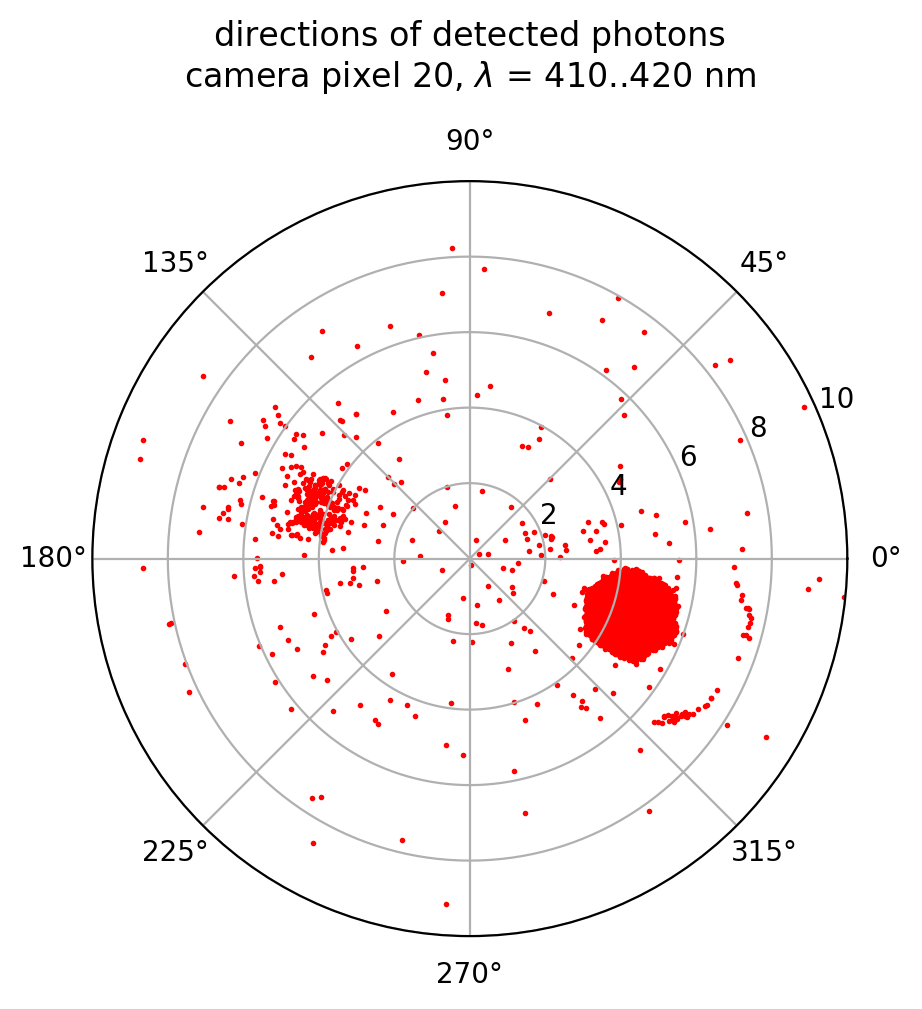
\includegraphics[width=0.5\textwidth]{scatter_px20_wvl410-420nm.png}
	\caption[Comparison: adaptive vs. non-adaptive KDE]{\textbf{Comparison: adaptive vs. non-adaptive KDE.} }
	\label{kde:example_scatter}	
\end{figure}

\begin{figure}
	\centering
	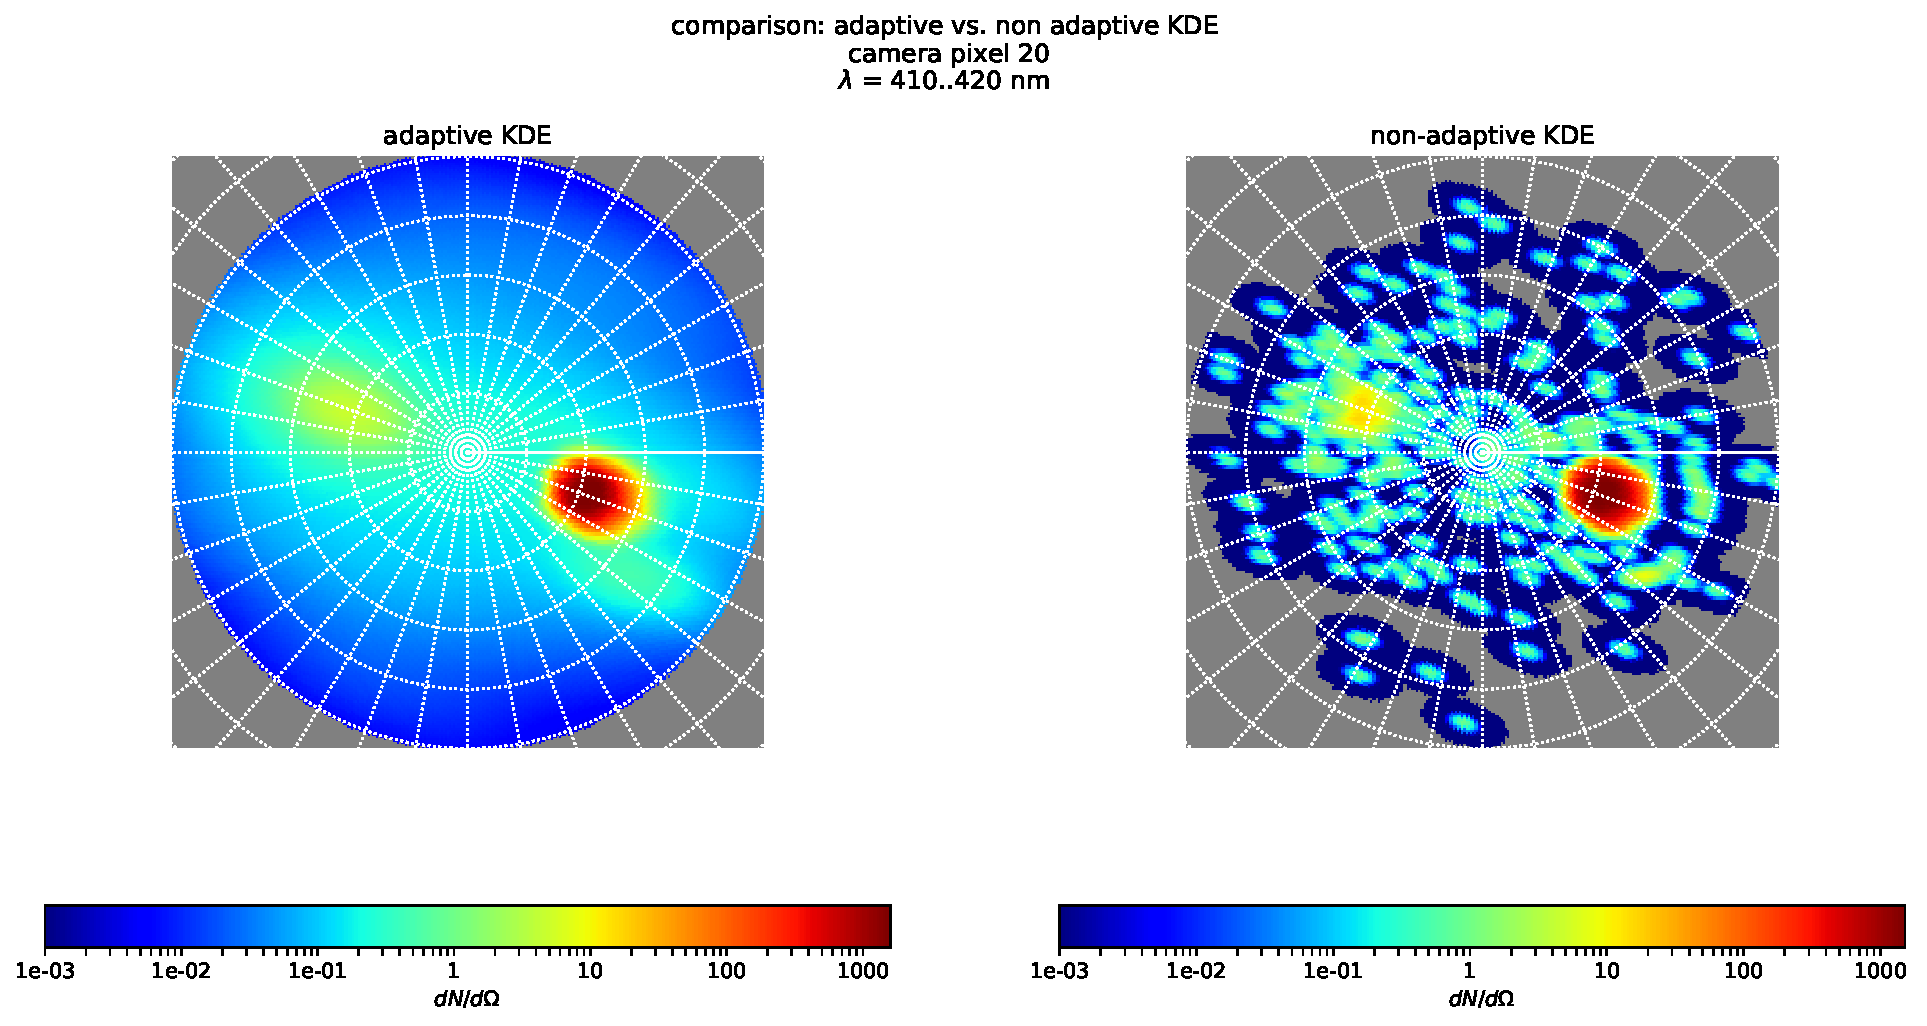
\includegraphics[width=\textwidth]{comparison_adaptive_nonadaptive.pdf}
	\caption[Comparison: adaptive vs. non-adaptive KDE]{\textbf{Comparison: adaptive vs. non-adaptive KDE.} }
	\label{kde:comparison}	
\end{figure}

\section{Detection Efficiency}

\subsection{The HEALPix Algorithm}

In order to account for the spherical shape of the angles of incidence it is useful to have angular bins with equal areas. Therefore, in this parameterization method, the \textit{HEALPix} (\textbf{H}ierarchical \textbf{E}qual \textbf{A}rea iso\textbf{L}atitude \textbf{Pix}elization) algorithm is used. It allows a uniform pixelization of incidence angles to the telescope.\\

\todo{healpix pixelization image}

The basic idea is to subdivide the sphere into 12 quadrilateral panes which can then further divided into more sub-panes as shown in figure \todo{figure reference}. A parameter $k$ numbers the subdivision step so that the number of sub-panes per each of the 12 panes is $N_{\text{side}}^2=\left(2^k\right)^2$. Hence, the total amount of pixels on the sphere is then
\begin{align}
N_\text{pix} = 12N_\text{side}^2\,.
\end{align}
Obviously, the angular resolution is dependent on $N_\text{pix}$, henceforth referred to as \enquote{pixel}.

\begin{table}[H]
\centering
\begin{tabular}{S[table-format=2.0]|S[table-format=4.0]|S[table-format=9.0]|S[table-format=2.2]}
\multicolumn{1}{l|}{$k$} & \multicolumn{1}{l|}{$N_\text{side} = 2^k$} & \multicolumn{1}{l|}{$N_\text{pix} = 12N_\text{nside}^2$} & \multicolumn{1}{l}{$\theta_\text{pix}$} \\
\hline
0  & 1    & 12        &  \SI{58.6}{\degree}\\
1  & 2    & 48        &  \SI{29.3}{\degree}\\
2  & 4    & 192       &  \SI{14.7}{\degree}\\
3  & 8    & 768 	  &  \SI{7.33}{\degree}\\
4  & 16   & 3072      &  \SI{3.66}{\degree}\\
5  & 32   & 12288     &  \SI{1.83}{\degree}\\
6  & 64   & 49152     &  \SI{55.0}{\arcminute}\\
7  & 128  & 196608    &  \SI{27.5}{\arcminute}\\
8  & 256  & 786432    &  \SI{13.7}{\arcminute}\\
9  & 512  & 3145728   &  \SI{6.87}{\arcminute}\\
10 & 1024 & 12582912  &  \SI{3.44}{\arcminute}\\
11 & 2048 & 50331648  &  \SI{1.72}{\arcminute}\\
12 & 4096 & 201326592 &  \SI{51.5}{\arcsecond}\\
13 & 8192 & 805306368 &  \SI{25.8}{\arcsecond}\\
\multicolumn{1}{c|}{\vdots} & \multicolumn{1}{c|}{\vdots} & \multicolumn{1}{c|}{\vdots} & \multicolumn{1}{c}{\vdots} \\
\end{tabular}
\caption[HEALPix parameters and resulting angular resolutions]{\textbf{HEALPix parameters and resulting angular resolutions.} $k$ represents the number of dividing iterations on the 12 panes, $N_\text{side}$ the number of tiles per pane edge, $N_\text{pix}$ the total number of pixels, and $\theta_\text{pix}$ the angular resolution defined by the angular length of a pixel edge. \cite{healpix:paper}}
\end{table}

For the application in this simulation the pixelization of a whole sphere is not needed since the telescope only has a field of view of about \SI{12}{\degree} (i.e. $\theta \leq \SI{6}{\degree}$). Considering that, one only needs a smaller sector of pixels around the zenith at $\theta = \SI{0}{\degree}$ which reduces the number of needed HEALPix by a factor of
\begin{align}
	2\pi\left(1-\cos\theta_\text{max}\right)\,.
\end{align}
For the IceAct simulation with $\theta_\text{max} = \SI{10}{\degree}$ this leads to the fact that only about $\SI{9.5}{\percent}$ of the HEALPixes are needed.

\section{Lookup Table}

\section{CORSIKA Implementation}\todo{vermutlich quatsch}
